\documentclass{article}
\usepackage[utf8]{inputenc}
\usepackage[spanish]{babel}
\usepackage{listings}
\usepackage{graphicx}
\graphicspath{ {images/} }
\usepackage{cite}
\usepackage[url]{hyperref}
\usepackage [latin1]{inputenc}
\begin{document}

\begin{titlepage}
    \begin{center}
        \vspace*{1cm}
            
        \Huge
        \textbf{Parcial 1 Informática II}
            
        \vspace{0.5cm}
        \LARGE
        Informe del desarrollo
            
        \vspace{1.5cm}
            
        \textbf{Luis Miguel Gil Rodrigez}
        \newline
        \textbf{Sebastian Giraldo Gómez}
        \newline
        \textbf{Maverick Sossa Tobón}
        \newline
            
        \vfill
            
        \vspace{0.8cm}
            
        \Large
        Despartamento de Ingeniería Electrónica y Telecomunicaciones\\
        Universidad de Antioquia\\
        Medellín\\
        Marzo de 2021
            
    \end{center}
\end{titlepage}

\tableofcontents
\newpage
\section{Sección introductoria}\label{intro}
Los establecimientos comerciales cada vez implementan mas técnicas que permiten su  crecimiento económico. Es claro que el cliente es uno de los factores más importantes (sino el que más), por lo que es necesario que cada interaccion que éste tenga con el negacio sea del mejor agrado posible, y una primera impresion suele cautivar a cualquiera. Entre muchas otras cosas, un buen letrero suele llamar la atención, es un indicador de calidad y prestigio. Es un aspecto importante que se queda en los recuerdos de los clientes. 
\newline

Se hace notoriaa la necesidad de innovar en este aspecto, ofrecerle a los negocios físicos un efectivo método que atraiga a los interesados.  

Entonces, se requiere de la creación de un sistema, combinando hardware y software, que de pie a la solución del problema planteado. En el desarrollo del mismo se emplearán unas herramietas en específico. Con leds, cables, resistencias y una protoboard se contruye una matriz de 8x8 leds. 
Tal matriz, por medio de un integrado 4HC595 y un arduino, se controla a voluntad. 

\section{Análisis del problema} \label{contenido}
Partiendo de una cantidad limitada de herramientas que se pueden implementar para la conexión del circuito, primero, se construye una matriz de leds de 8 x 8, con sus respectivas resistencias, la cuala será controlada por dos integrados 74HC595. Un integrado maneja la parte de las filas y otro integrado las columnas. Por motivos de orden y practicidad, se utiliza una protoboard para hacer el cableado al arduino para despues hacer 
\newline

Inicialmente se observa que se puede conectar los integrados en paralelo, para que la señal de entrada a un integrado principal, comprometa la salida del otro integrado. De esta manera manejamos las filas y columnas de la matriz de leds 8x8.
Para el control de esta matriz se crean arreglos con notación binaria y hexadecimal las cuales representan los estados de los leds, es decir, encendido (1) o apagado (0).
\newline

Una vez establecida la conexión entre los leds y el arduino y la forma del arreglo, se procede a programar un menú.
Se le presenta al usuario un menú de 3 opciones inicialmente, y entre algunas de éstas se despliegan otras. Lo adecuado sería hacer un switch case para que el usuario ingrese por el puerto serial un numero que representa la opción de aquello que desea hacer. 
\newline

En la opción en que el usuario ingresará un patrón cualquiera que desea ver, se deberá tener en cuenta que cada uno de los ocho numeros representa una fila de la matriz. La forma en como se va a encender una fila para un numero dado está basada en la representación binaria de tal numero. Los ocho (8) bits que lo conformen indican cuales leds estarán encendidos (1 para encedido y 0 para apagado) empezando con el bit menos significativo. 
Entonces a la hora de querer un patrón en específico, es importante que previamente se identifique qué numeros, y en qué orden, son los que podrán dar como resultado el patrón buscado. 

\section{Diagrama de tareas}
Dado que la longitud del código del programa es un tanto extensa, y que para tener una idea general de la estructura del mismo es necesario leerlo, resulta práctico tener un diagrama que ilustre, brevemente, el funcionamiento del programa. Esto como una alternativa a leer la documentación del código.

\begin{figure}[h!]
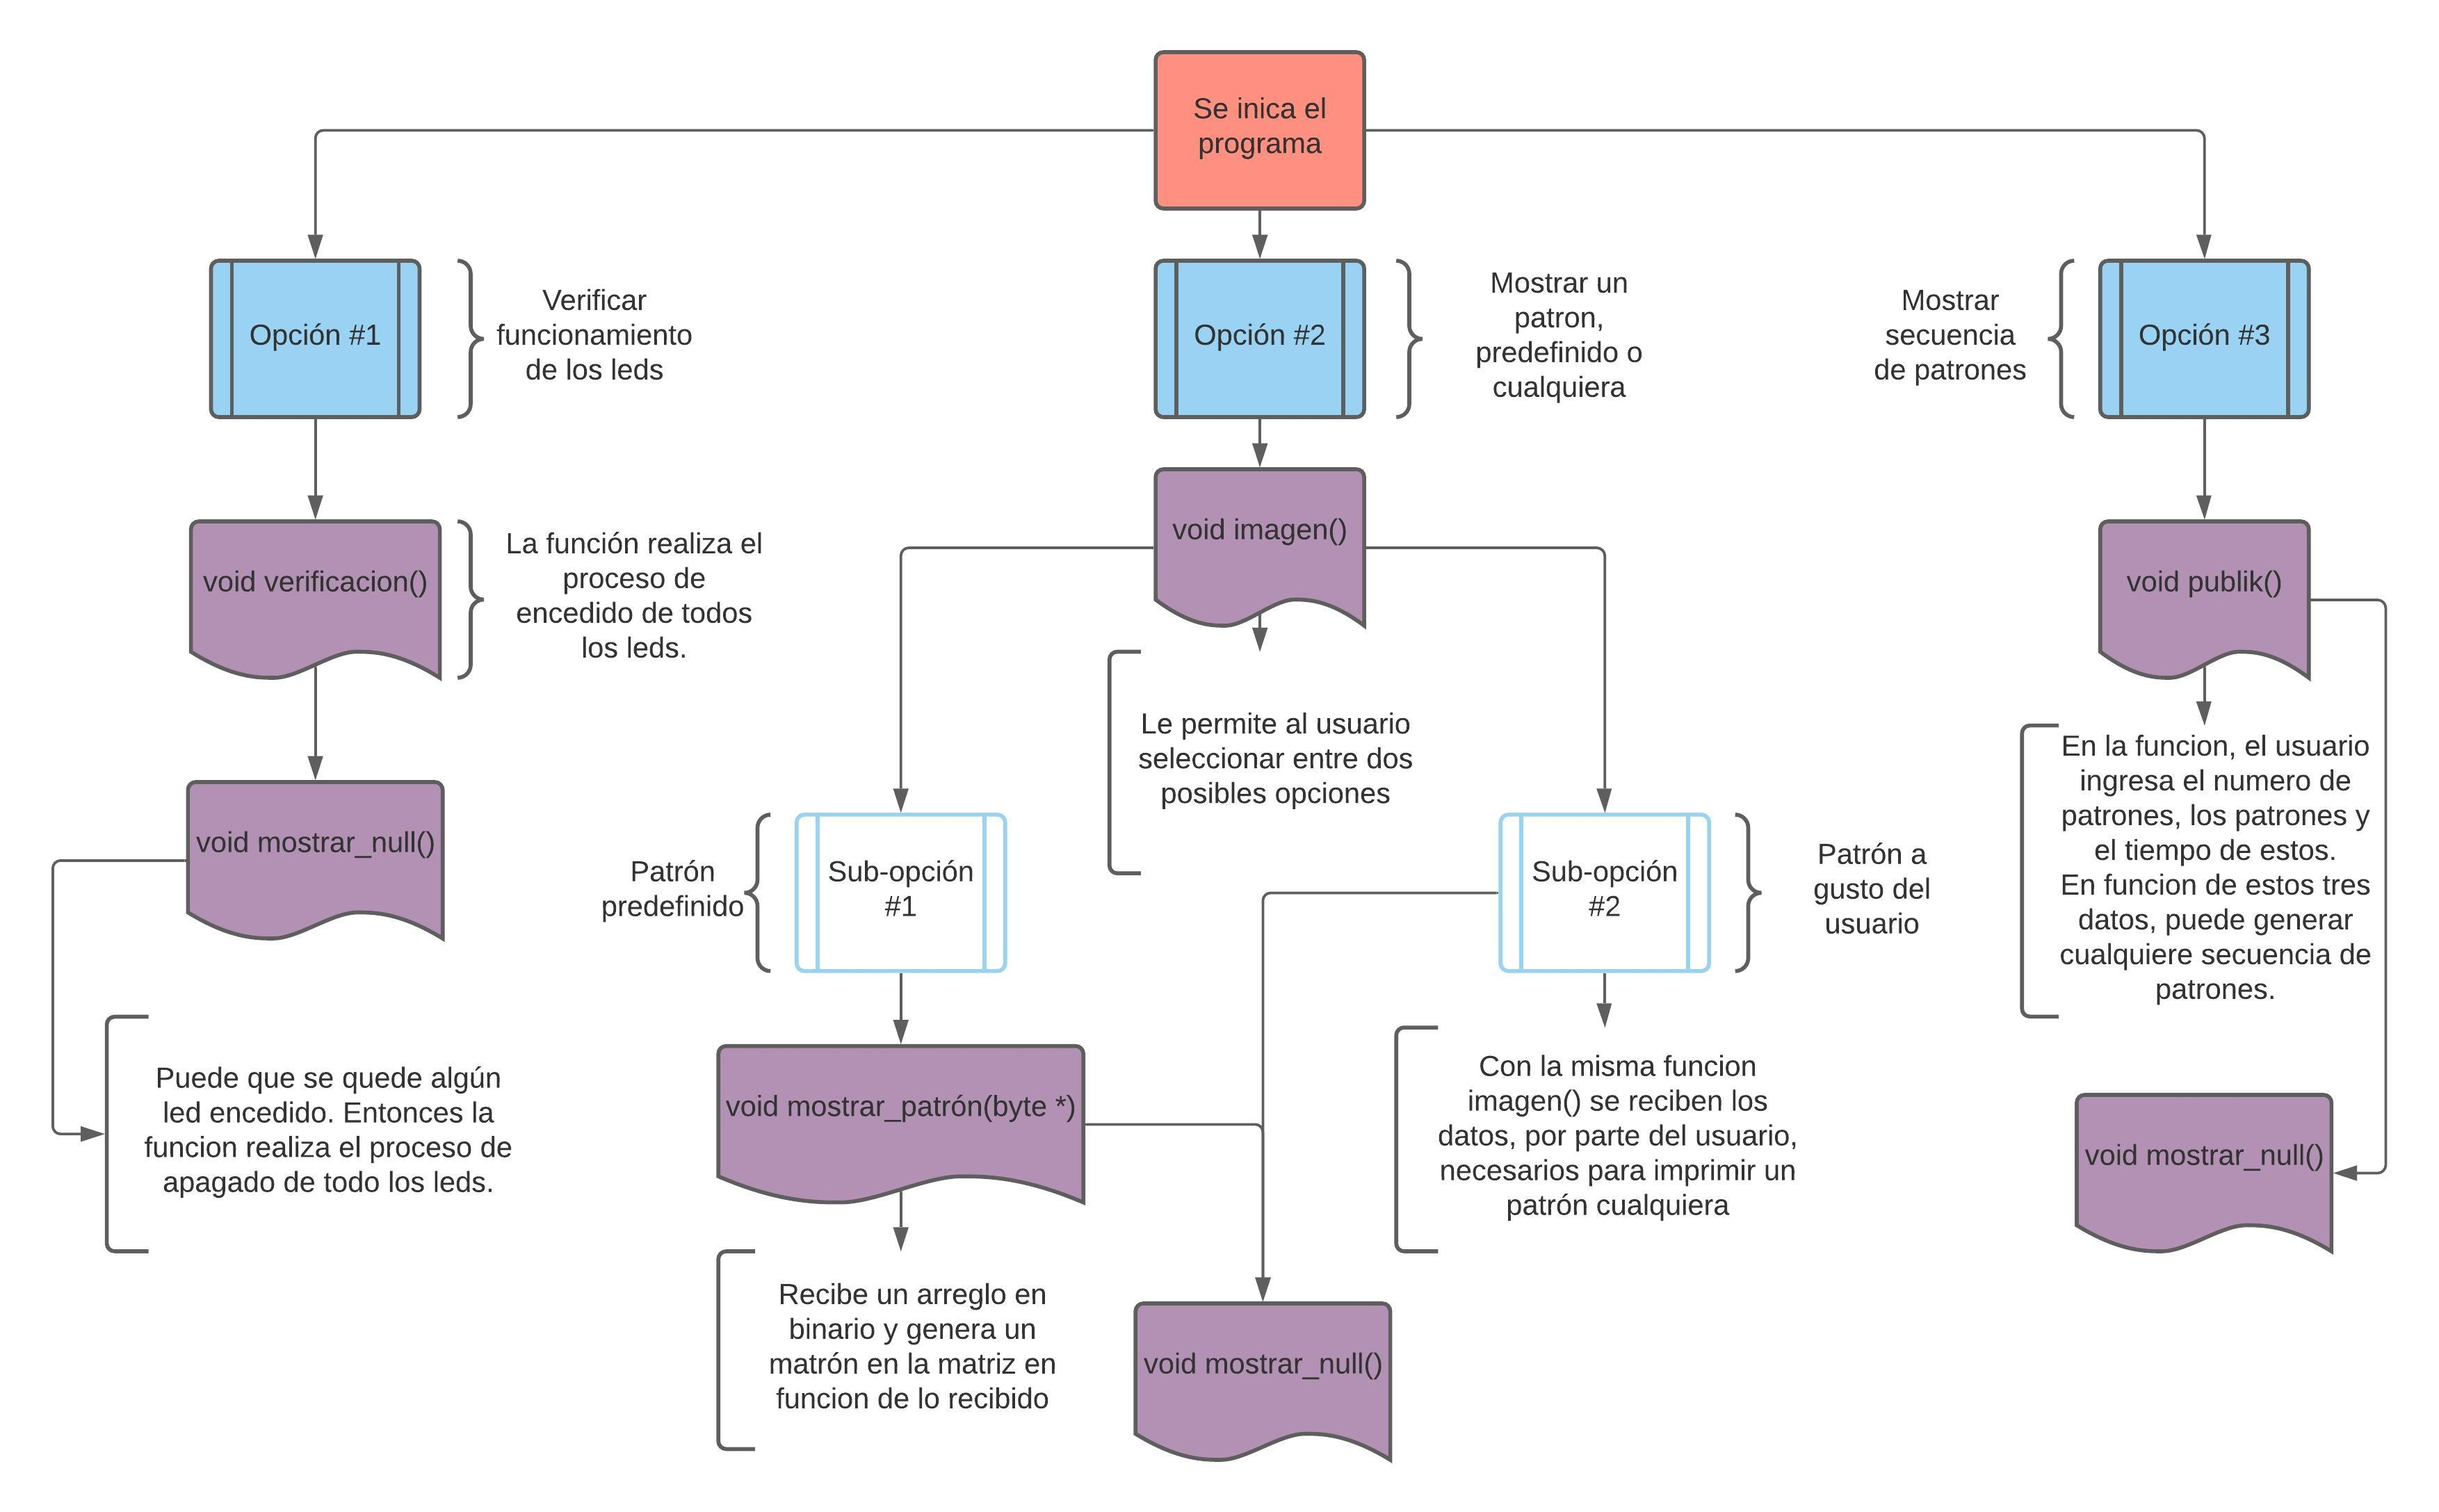
\includegraphics[width=13cm]{Diagrama de tareas.jpeg}
\centering
\caption{Diagrama}
\label{fig:Diagrama}
\end{figure}

\section{Algoritmo implementado}
Para cumplir con un objetivo, resulta prático elaborar un plan en el que se establezca el modo y los medios disponibles y necesarios para llevar a cabo tal fin. Desarrollar un algoritmo, en donde se plantee un conjunto de pasos ordenados que permiten obtener cierto resultado buscado, es de las mejores formas de trazar el camino a seguir. Además, si se redacta, brevemente, la estructura del algoritmo implementado en la solución del problema puede ayudar a tener una idea general del método de solcuión empleado. 

\begin{lstlisting}[language=C++, label=codigo_ejemplo]
// Protipo de funciones. 
void verificacion();
void imagen();
void publik();
void mostrar_patron(byte *);
void mostrar_null();

// Se crean e iniciliazan varibles globales tipo int y byte
const int data = 2;
const int store = 3;
const int shift = 4;
int opt; // Entre otras

void setup() {
    // Se incializa los puertos digitales (3) y serial
}
void loop() {
    // Imprime las opciones del menu principal
    Serial.println("Menu");
    // Se recibe el numero ingresado por el usuario
    opt = Serial.parseInt();
    // Con un switch, se hace algo segun lo ingresado
    switch(opt){
    case 1:
        // See invoca la funcion verificacion, 
        // la cual enciende todos los leds
        verificacion();
    case 2:
        // Se invoca la funcion imagen, para 
        // mostrar un patron de leds
        imagen();
    case 3:
        // Se invoca publik, que se encarga de 
        // mostrar una secuencia de patrones
        publik();
    default:
        // Caso de dato ingresado fuera de rango. 
    }
}
void mostrar_null() {
    // La funcion pone todos los leds en apagado (0)
    for (int i = 0; i<8; i++) {
        // Itera sobre cada fila de la matriz de leds
    }
        
}
void mostrar_patron(byte *arreglo) {
    // Genera un patron ingresado por el usuario
    for (int k = 0; k<20; k++) {
        // Itera sobre el tiempo a mostrar el patron
        for (int i = 0; i<8; i++) {
            // Itera sobre cada fila de la matriz
        }
    }
    mostrar_null(); // Se apaga todo 
}
void verificacion() { // Enciende todo los leds
    // La variable global 'all' contiene un arreglo que 
    // permite encenderlos todos por medio de la funcion
    mostrar_patron(all);
}
void imagen() {
    // Se imprime el submenu
    Serial.println("Sub-menu");
    // Se le pide al usuario seleccionar una opcion
    int opt2;
    opt2 = Serial.paseInt();
    switch(opt2) {
    case 1:
        //Opcion de patron predefinido
        char caracter;
        // Se ingresa el caracter del patron
        caracter = Serial.read();
        // Despues hay un largo else if para saber 
        // que patron mostrar
        if (caracter == 'A')
            mostrar_patron(A);
        else if (caracter == 'B')
            mostrar_patron(B);
        ...
        ...
        ...
    case 2:
        int patron[8];
        // Opcion de patron ingresado por el usuario
        for (int i = 0; i<8; i++) {
            // Itera sobe las 8 filas
            // Se agrega a 'patron' cada fila
            *(patron + i) = Serial.parseInt();
        }// Despues de ingresados las 8 filas, se muestra el patron
        for (int k = 0; k<20; k++) {
            // Itera sobre el tiempo a mostrar el patron
            for (int i = 0; i<8; i++) {
                // Itera sobre cada fila de la matriz
            }
        }// Se apagan todos lo leds
        mostrar_null();
    default:
        // Para el caso de opcion fuera de rango. 
    }
}

void publik() { // Mustra una secuencia de patrones. 
    int num_patrones = 0; // Cantidad de patrones a mostrar
    int num = 0; // 
    // El usuario ingresa la cantidad de patrones
    num_patrones = Serial.parseInt();
    // Se crea dinamicamente un arreglo que contendra 
    // los patrones a mostrar
    int **secuencias = new int *[num_patrones];
    for(int i = 0; i < num_patrones; i++){
        // Cada elemento es una patron
        secuencias[i] = new int [8];
    }for (int i = 0; i<num_patrones; i++) {
        // Itera sobre cada patron
        for (int j = 0; j<8; j++) {
            // Itera sobre cada fila
            // El usuario ingresa cada fila 
            num = Serial.parseInt();
            while ((num > 255) || (num < 0)) {
                // Se verifica que la fila ingresada 
                // pertenezca al rango valido
                num = Serial.parseInt();
            }// Se agrega la fila al arreglo
            secuencias[i][j] = num;
        }
    }// Fin del ingreso de valores al arreglo de secuencias
    // El usuario ingresa el tiempo entre patrones
    int tempo = Serial.parseInt();
    int cont_secuencia = 0;
    while (cont_secuencia != num_secuencia) {
        // Itera sobre cada patron
        for (int k = 0; k<20; k++) {
            // Intera sobre la cantidad de veces que se 
            // muestrar cada patron 
            for (int i = 0; i<8; i++) {
                // Itera sobre cada fila de un patro
                delay(tempo);
            }
        }cont_secuencia++;
    }// Fin de mostrar la secuencia de patrones
    mostrar_null(); // Se apagan todos los leds
    // Se borra del heap las secuencia de patrones 
    delete []secuencias;
}


\end{lstlisting}
\section{Problemas de desarrollo en el proceso}
En el proceso de solución de un problema, por lo general, se presentan dificultades o retos que realentizan la culminación del mismo. Es claro que el haber superado tales obtáculos en el camino, resulta ser algo muy enriquecedor y satisfactorio, por lo que, más que un estorbo, son realmente el dasafío más grande, y el logro de haberlos afrontado resulta en un trofeo incluso más grande que el de la propia consecución del proyecto principal. 
\newline
Se enuncian a continuación los retos más destacado en el desarrollo. 
\begin{enumerate}
    \item 
    Confusión a la hora plantear un modelo circuital, pues no hay seguridad de que lo que se realice cumpla con el objetivo.
    \item 
    Confusión para generar un patrón a partir de la estructura general planteada para el programa. 
    \item
    La plataforma tinkercad pone problemas para la ejecución del código, realentizando las pruebas al programa y la elaboración del mismo. 
    \item
    La velocidad de ejecución del programa en Tinkercad depende altamente del computador en el que se corre éste, por lo que tarda en responder para la evaluación del circuito.
\end{enumerate}

\section{Evolución del algoritmo}
\begin{enumerate}
    \item 
    Se procede a programar el código para la lectura de los puertos digitales del Arduino
    \item
    Se hace programa para recorrer la matriz de leds y por ende mostrar la verificación de la matriz de leds.
    \item
    Se crea la función imagen y se agregan patrones predefinidos. Para los patrones predefinidos se visita la siguiente pagin \href{https://rodrigosc.github.io/ArduinoLedMatrix/char_builder/builder.html}{Character Builder}. La cual genera la matriz de 8x8.
    \item
    Se crea un menú para que el usuario pueda escoger un patrón predefinido o el usuario ingrese un patrón.
    \item
    Se crea la función publik en la cual el usuario puede ingresar varias secuencias de patrones.
    \item
    Debido a la longitud del código, se crea la función “mostrar patrón” para disminuir la cantidad de líneas en el código.
    \item
    En periodo de pruebas, se evidencia que al mostrar por los leds un patrón que encienda al menos un led de la última fila, esta fila quedará encendida. Por lo tanto se procede a programar una función “mostrar null” que apaga esta última fila encendida.
    
\end{enumerate}

\end{document}
